\chapter{Implementation}
\section{Overview}
This chapter focuses on the practical aspects of implementing a student evaluation system in educational institutions. It explores the key considerations, strategies, and steps involved in effectively implementing such systems.  After designing the system and implementation, the ultimate results are shown here with all the details. This project is aimed at developing an efficient online student evaluation system for the university students.



\section{Practical Implementation}
In this project, there has been used HTML,CSS and Javascript to design the website pages for user’s interface. On our system, there will be two login systems both for the teachers and the students. To login into the system both users have to sign up to open their account. These accounts will be confirmed by the university admin after checking the information. In the following figure
\ref{fig:home} the login interfaces are given:
\begin{figure}[H]
    \centering
    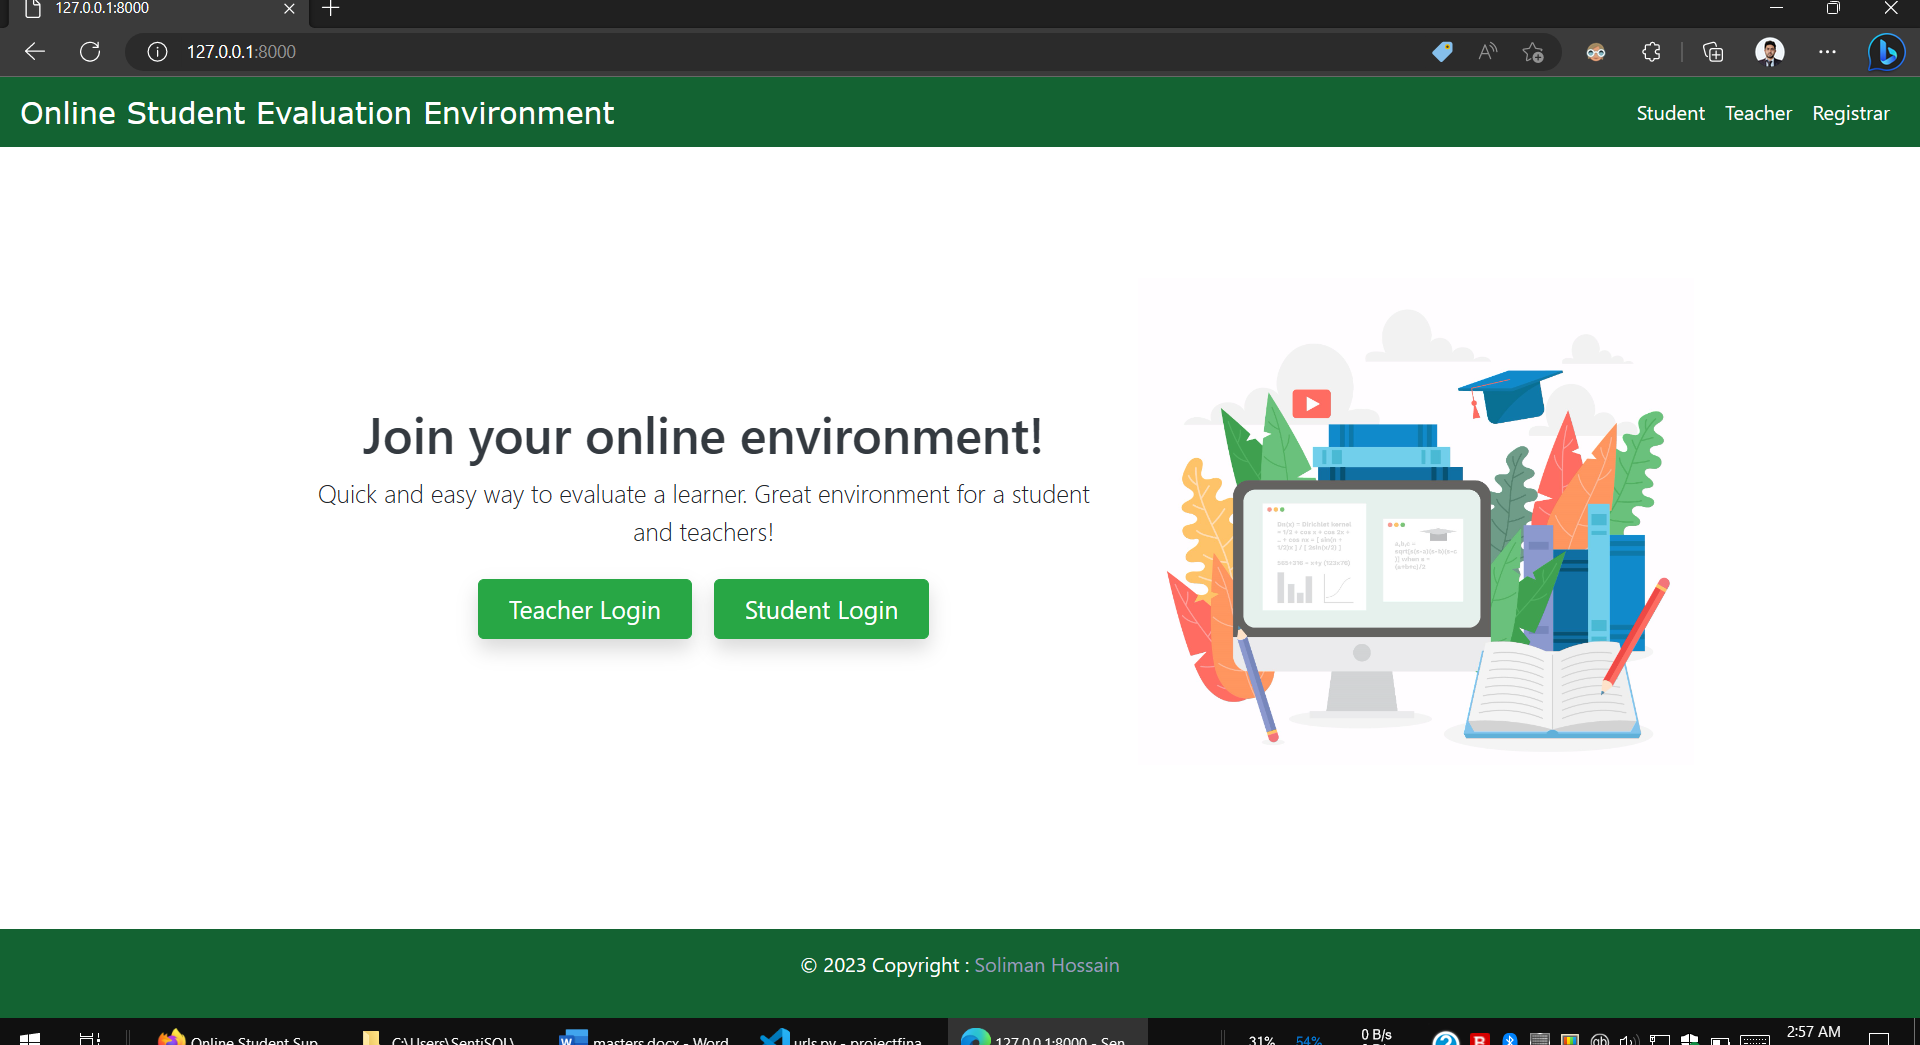
\includegraphics[scale=.35]{img/home.png}
    \caption{Home Interface}
    \label{fig:home}
\end{figure}

\subsection{Student}
Before login a student will need to sign up by providing some information about him/her which is only done by Registrar. This information will help to recognize him/her as a unique ID which will confirm he/ she is the student of that particular university. The following figure \ref{fig:stduentsign} shows what exact information a student will need to provide during sign up or creating the account.
\begin{figure}[H]
    \centering
    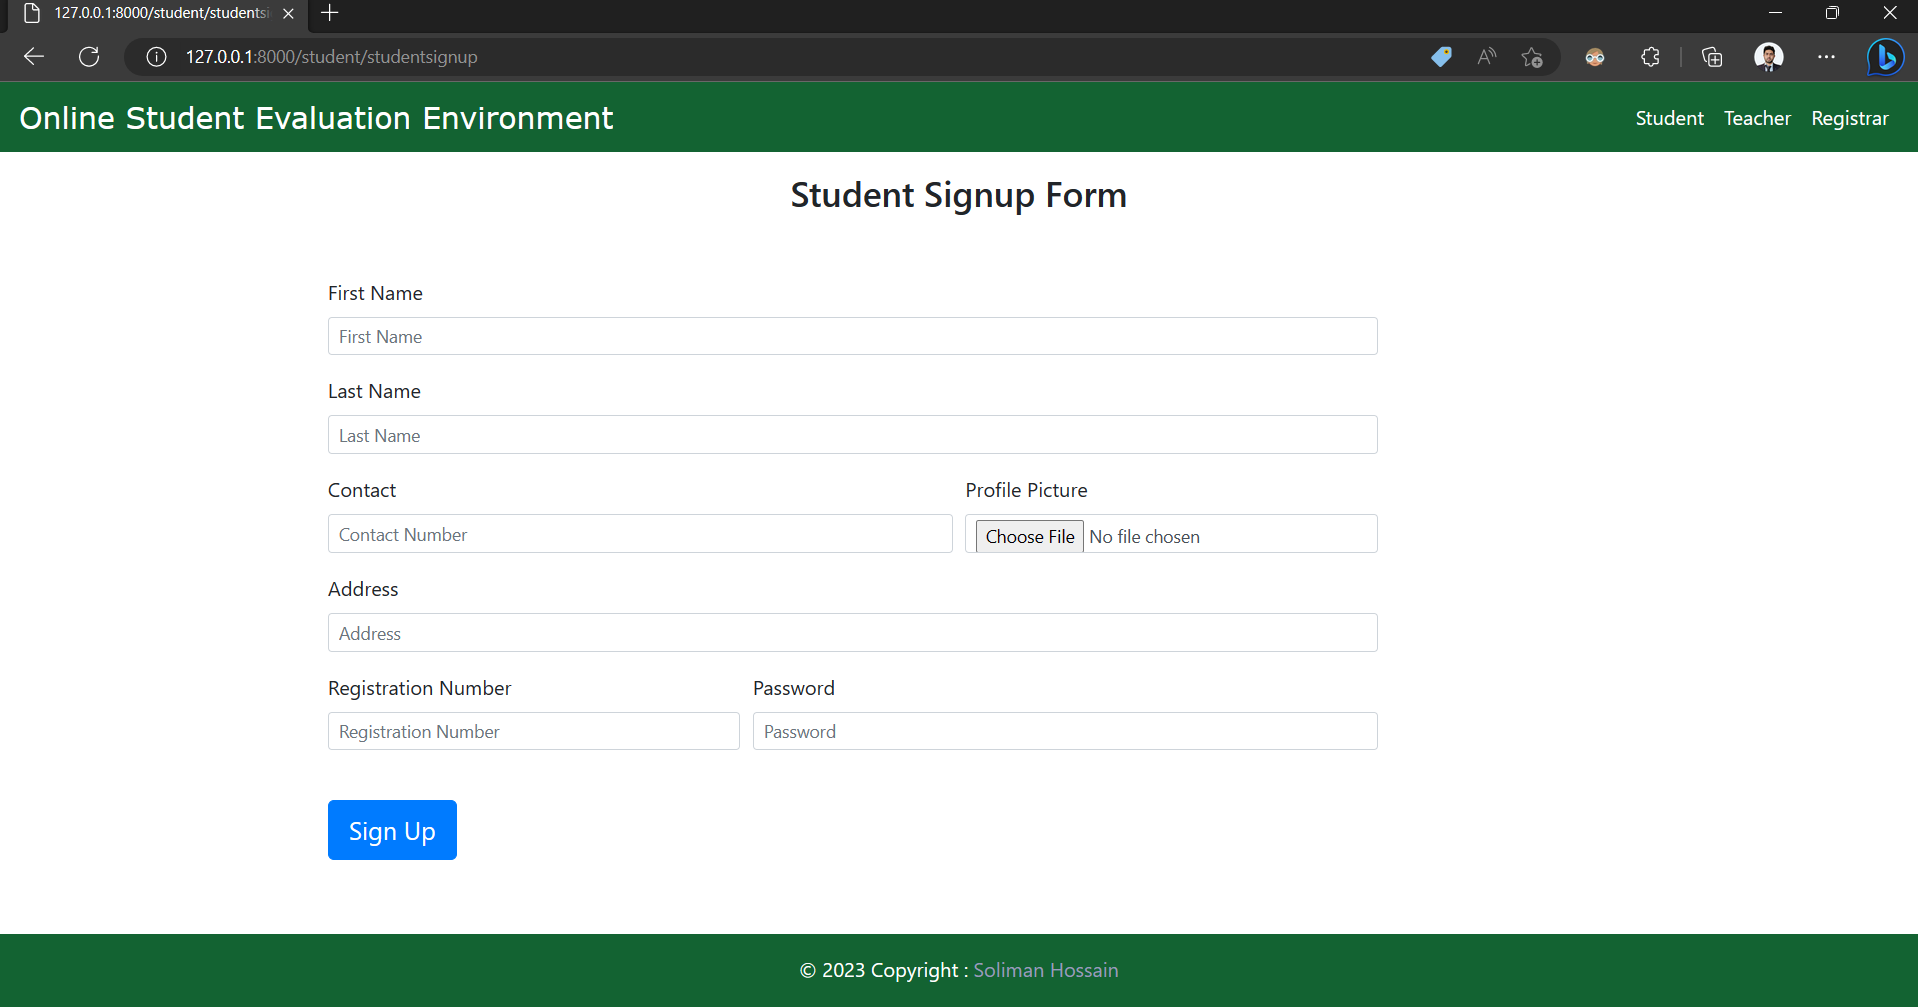
\includegraphics[scale=.35]{img/stduentsign.png}
    \caption{Student Sign-up Form}
    \label{fig:stduentsign}
\end{figure}
In the following figure \ref{fig:stduentlogin} it shows that during logging into the system, the student will need to give their own registration number and the password which he/she set up during creating the account. This registration number will be unique as it is provided by the university authority to every student. 
\begin{figure}[H]
    \centering
    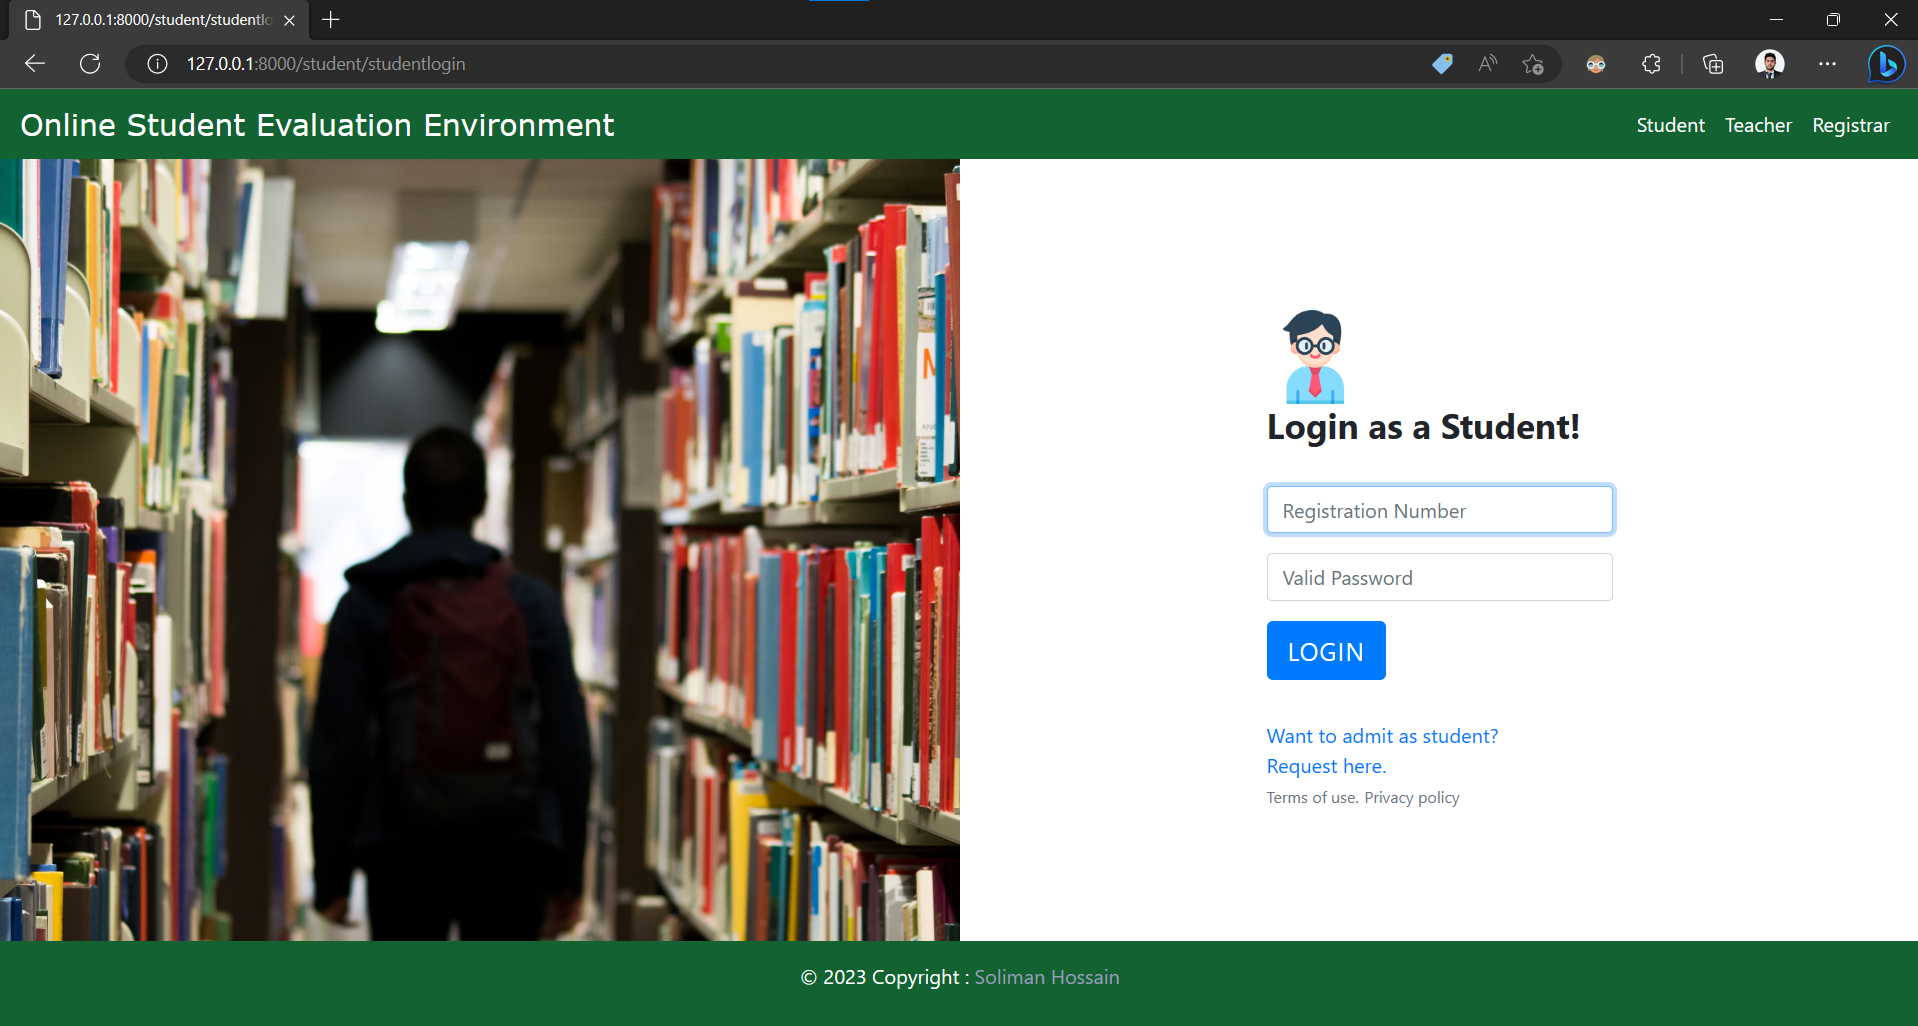
\includegraphics[scale=.35]{img/stduentlogin.png}
    \caption{Student login interface}
    \label{fig:stduentlogin}
\end{figure}
After successful login into the system a student will find on dashboard, the attached exams and total questions assigned to him as the following figure 4.4:
\begin{figure}[H]
    \centering
    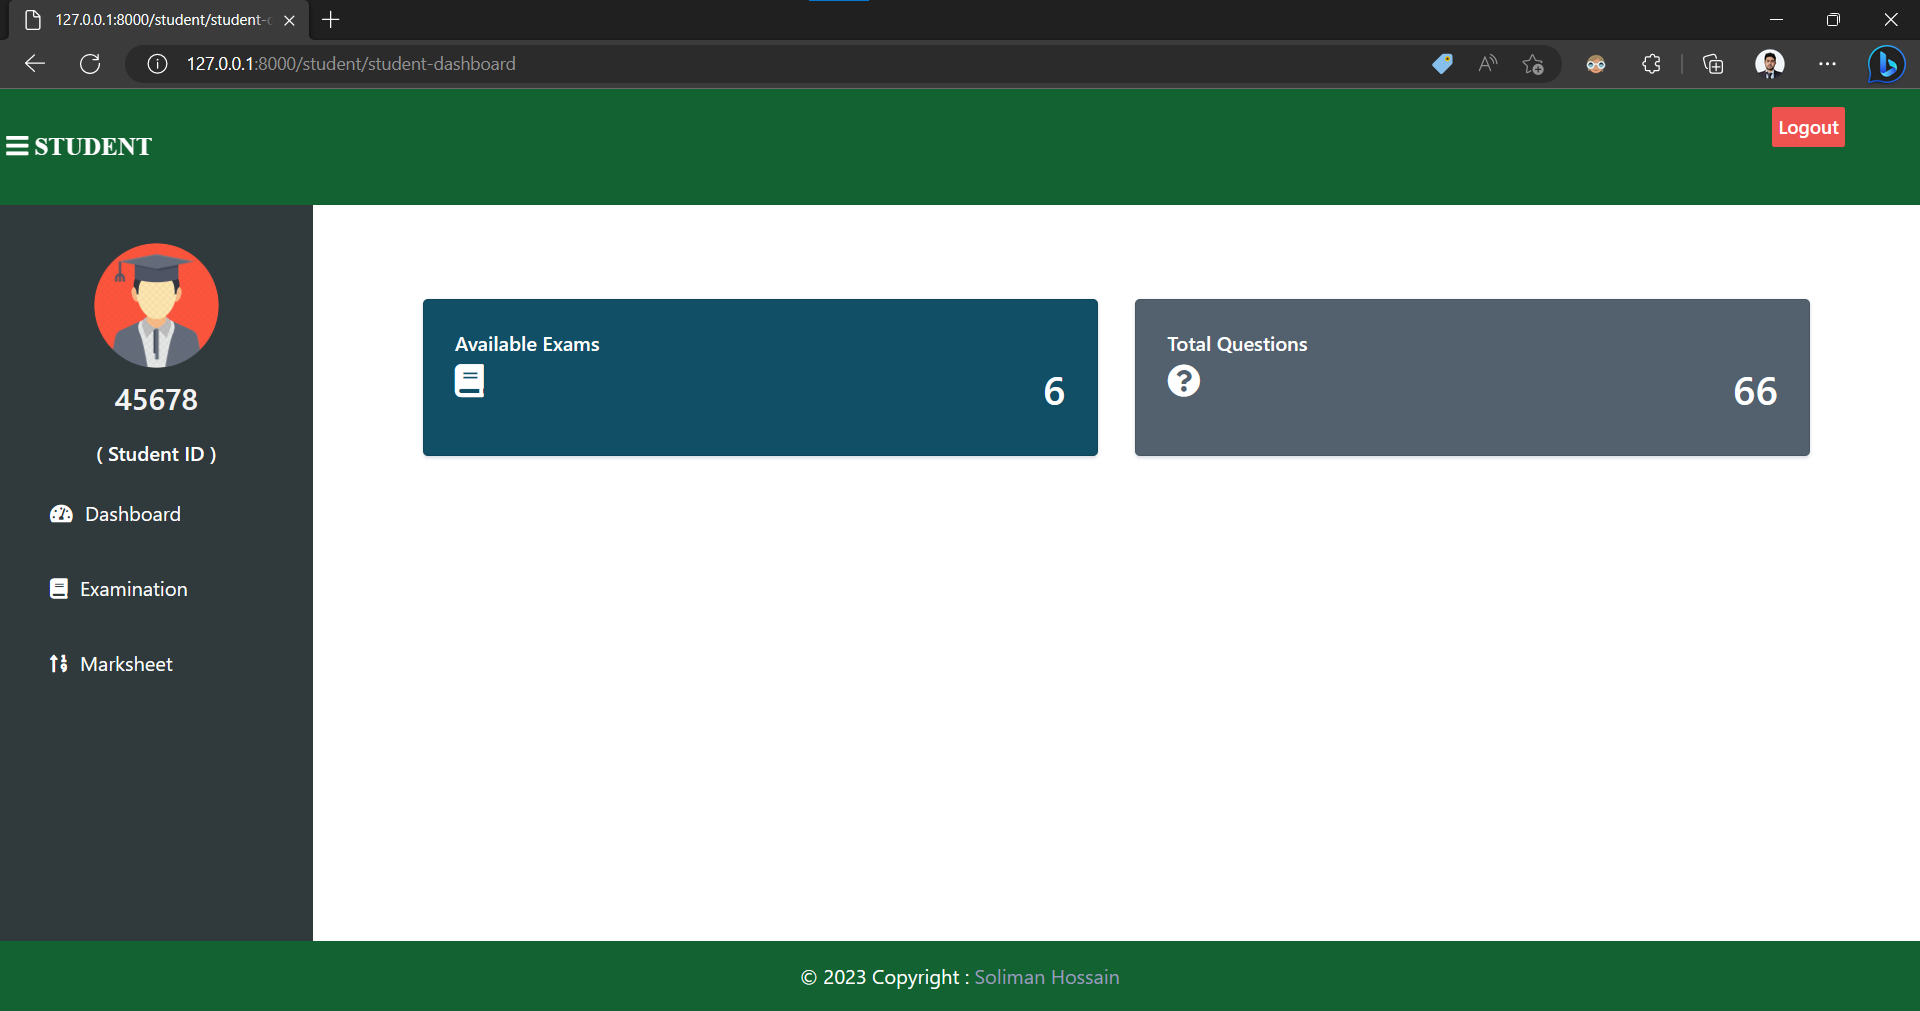
\includegraphics[scale=.35]{img/studentd.png}
    \caption{Student Profile}
    \label{fig:studentd}
\end{figure}

From the above interface the student will be able to show the questions, tasks which will be assigned to him at different times. Students will be able to show their exam marks and mistakes they have made during the exams. Additionally, they can upload their answer sheet as a pdf format when the answer sheets are written ones.
\ref{fig:stMCQ}and \ref{fig:stCT}.
\begin{figure}[H]
    \centering
    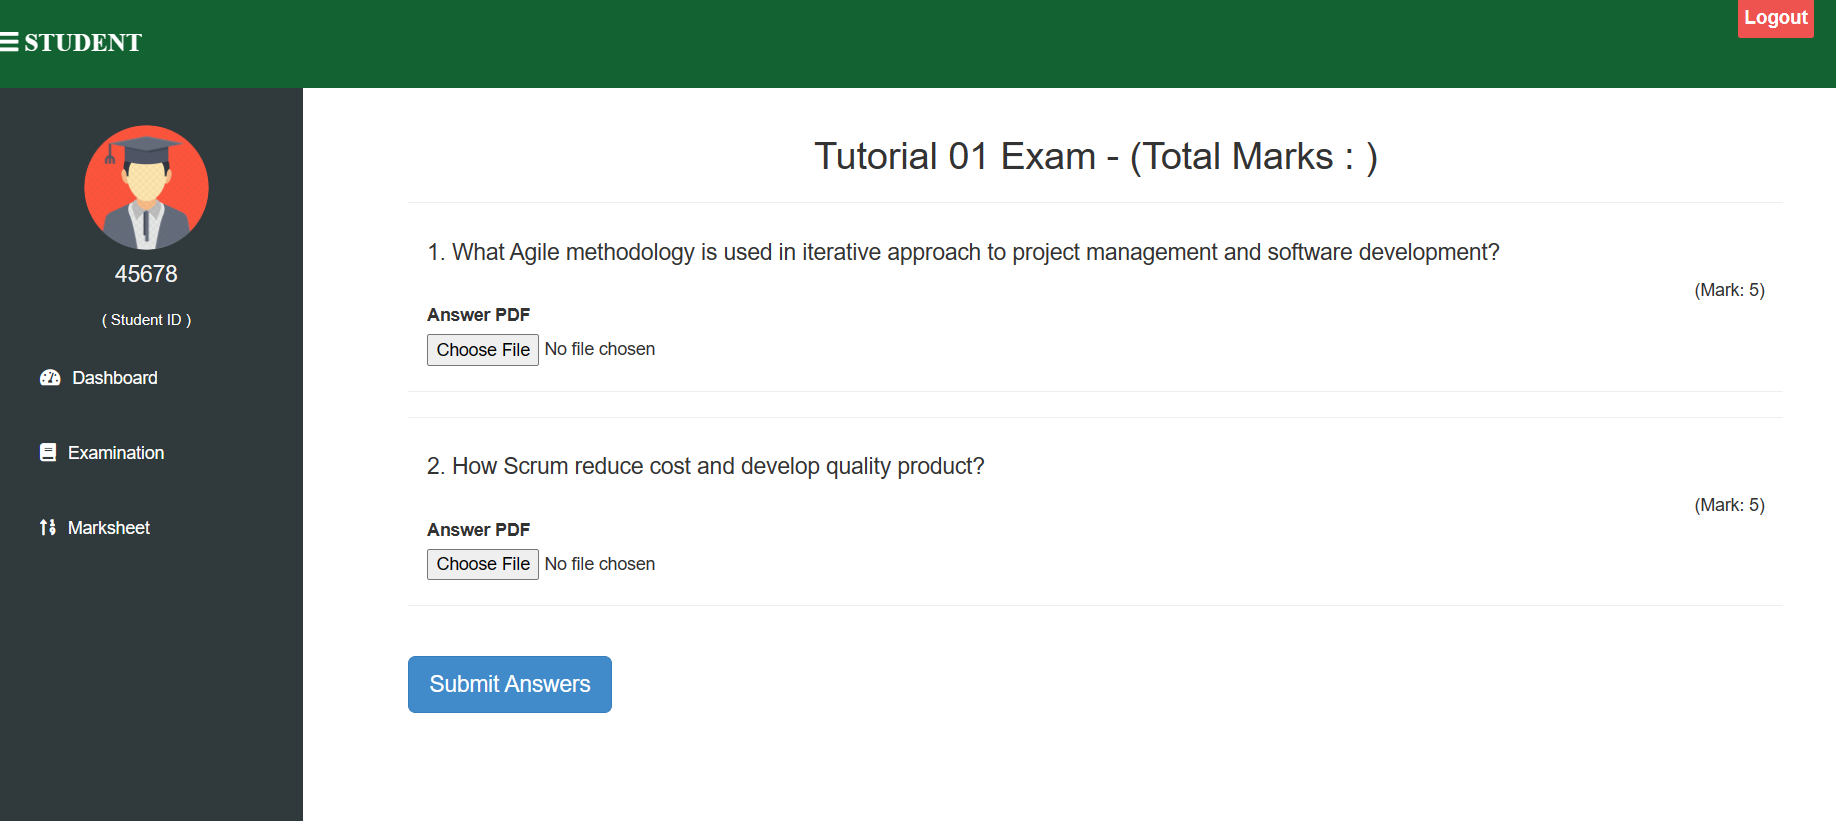
\includegraphics[scale=.35]{img/stCT.png}
    \caption{Written Exam}
    \label{fig:stCT}
\end{figure}
The student will be able to attend MCQ and written exams by using this platform and the evaluation of their tasks will be done by local browser cookies and machine learning techniques accordingly. The exam patterns on the platform are shown on the figure 
\begin{figure}[H]
    \centering
    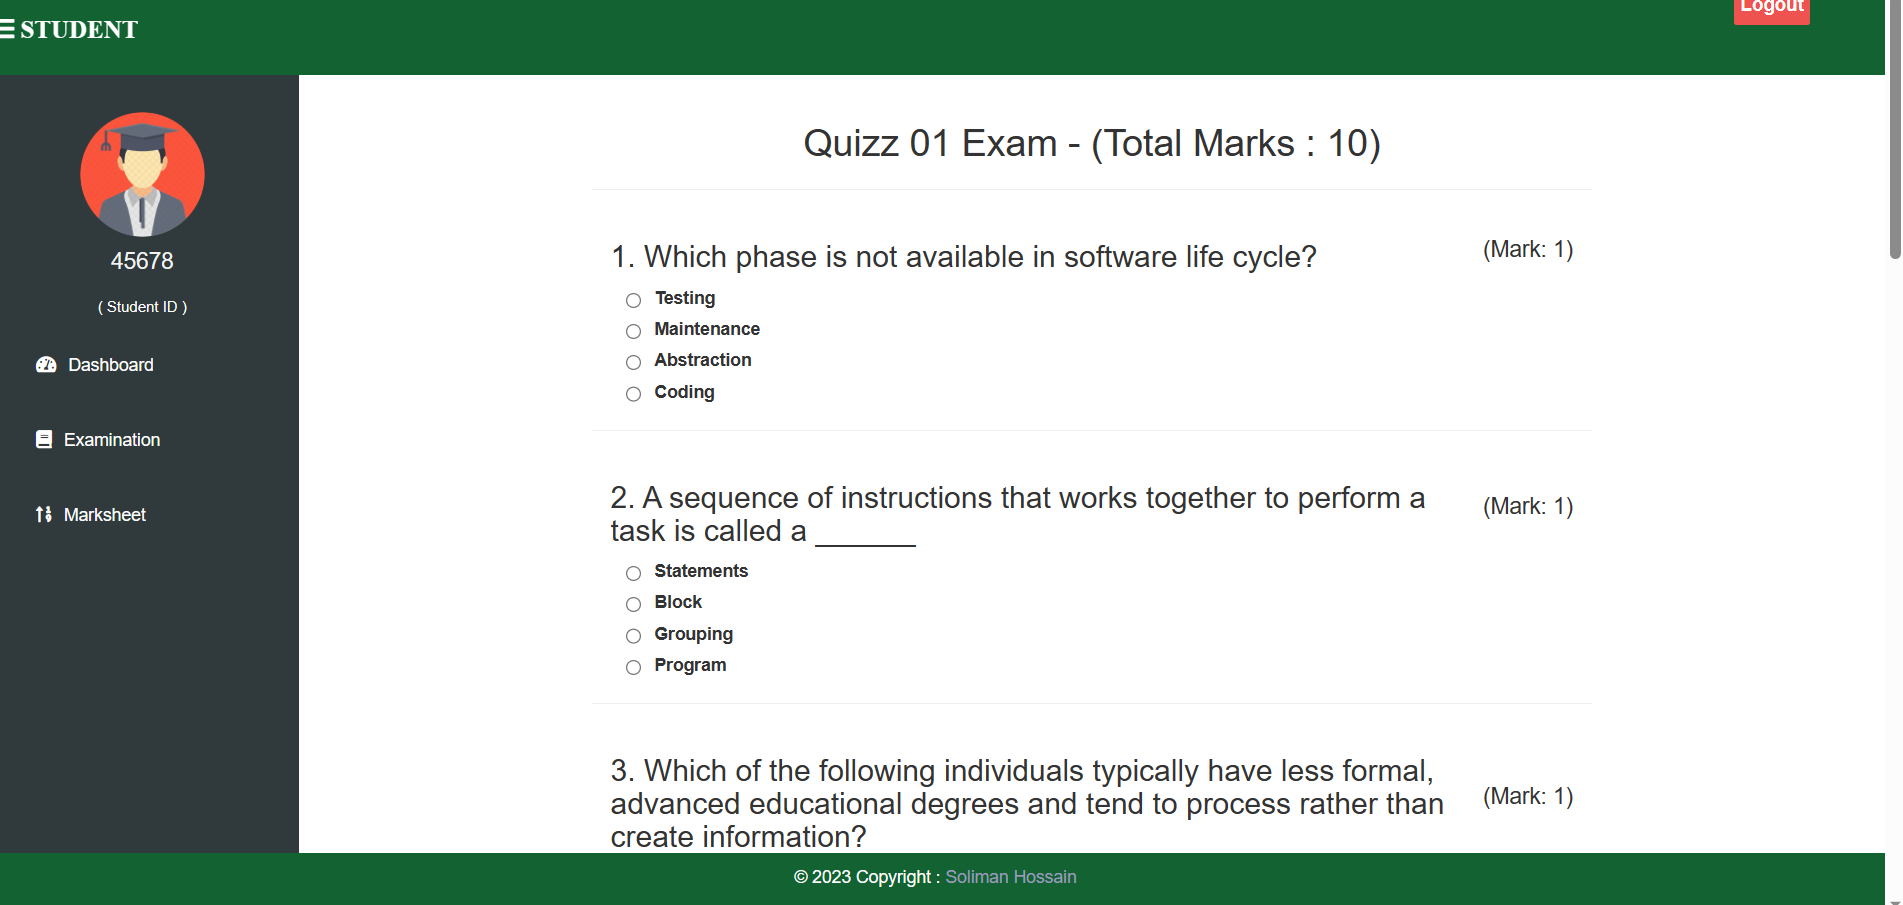
\includegraphics[scale=.35]{img/stMCQ.png}
    \caption{MCQ Exam}
    \label{fig:stMCQ}
\end{figure}

% \newpage
\subsection{Teacher}
As it is said that there will be two users so the teacher also needs to sign up and login into the system to follow up with the student’s tasks and exams. To create an account the teacher also will need to provide some information regarding the profession. The following figure \ref{fig:teacherup} shows the information which they will need to provide:
\begin{figure}[H]
    \centering
    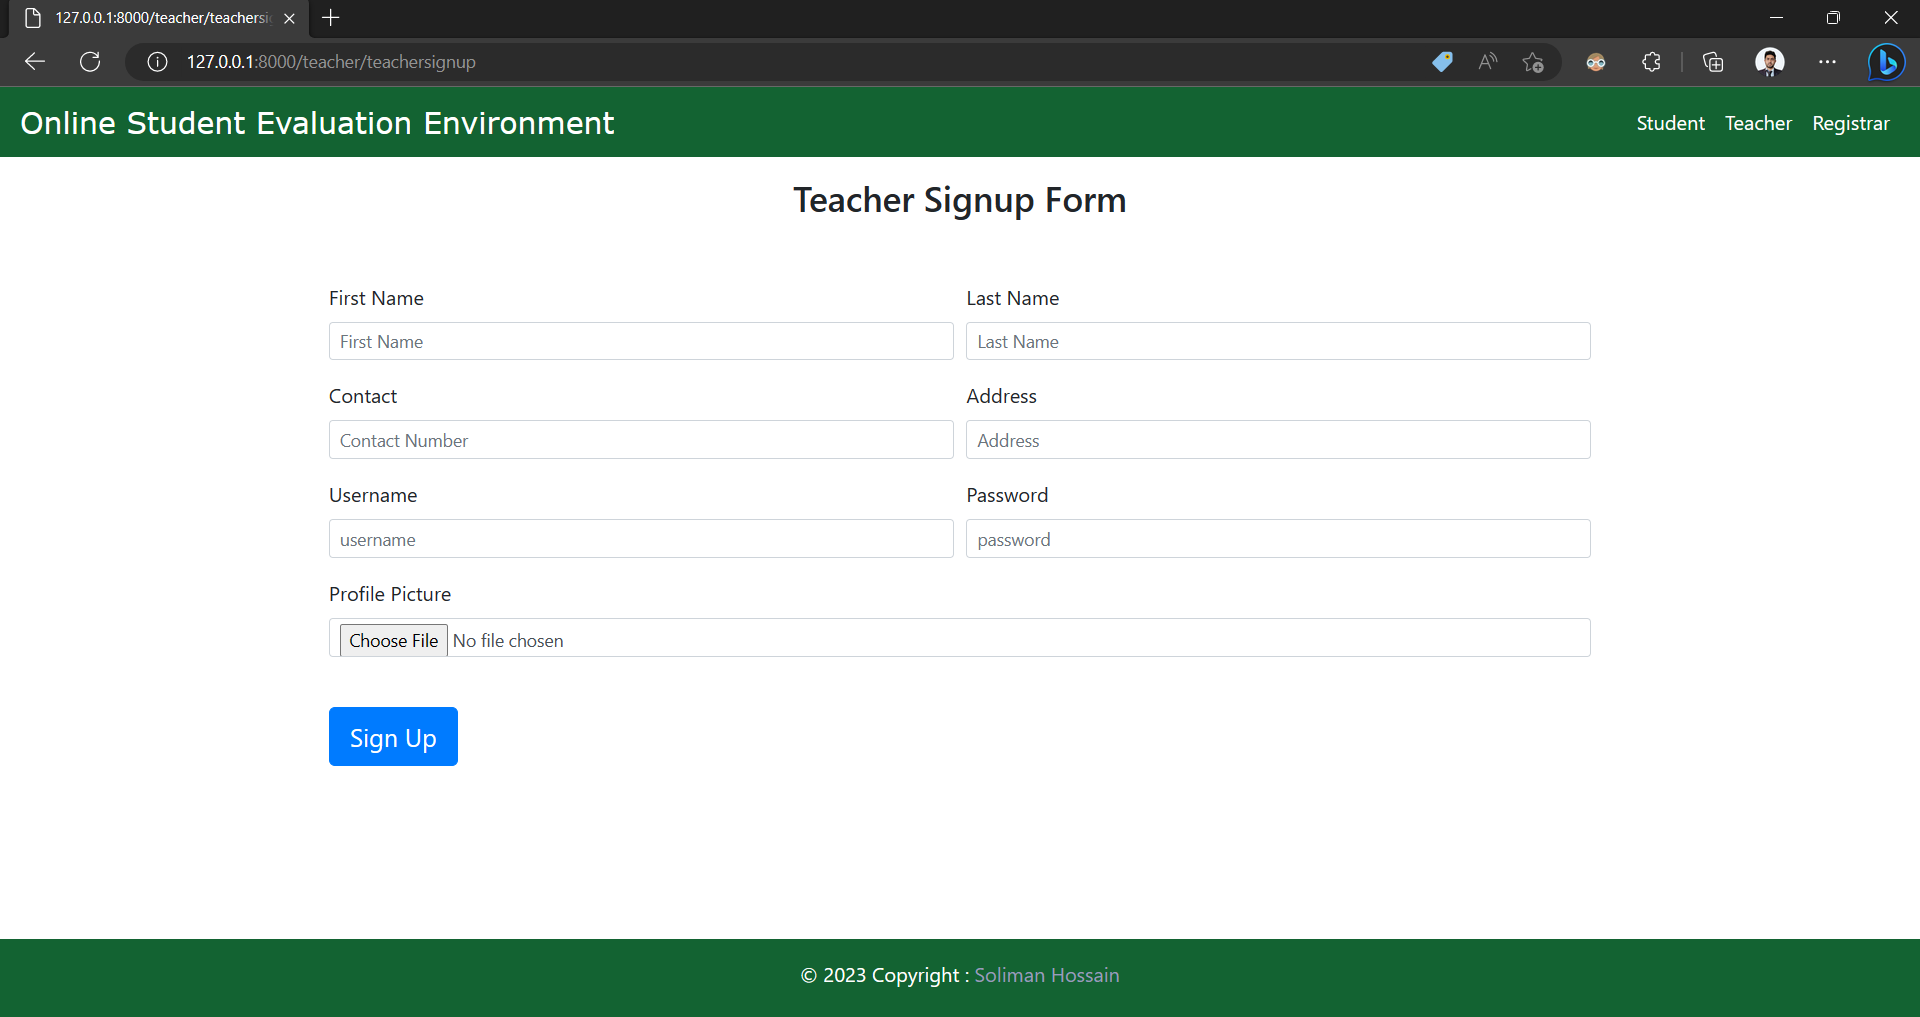
\includegraphics[scale=.35]{img/teacherup.png}
    \caption{Teacher Sign-up Form }
    \label{fig:teacherup}
\end{figure}
During login into the system the teacher will need to provide their username and the password which he/she set up in the sign up form. After login to the system, the teacher will be able to see the students list and also it will be possible to upload the question for both the written and MCQ exams.
\begin{figure}[H]
    \centering
    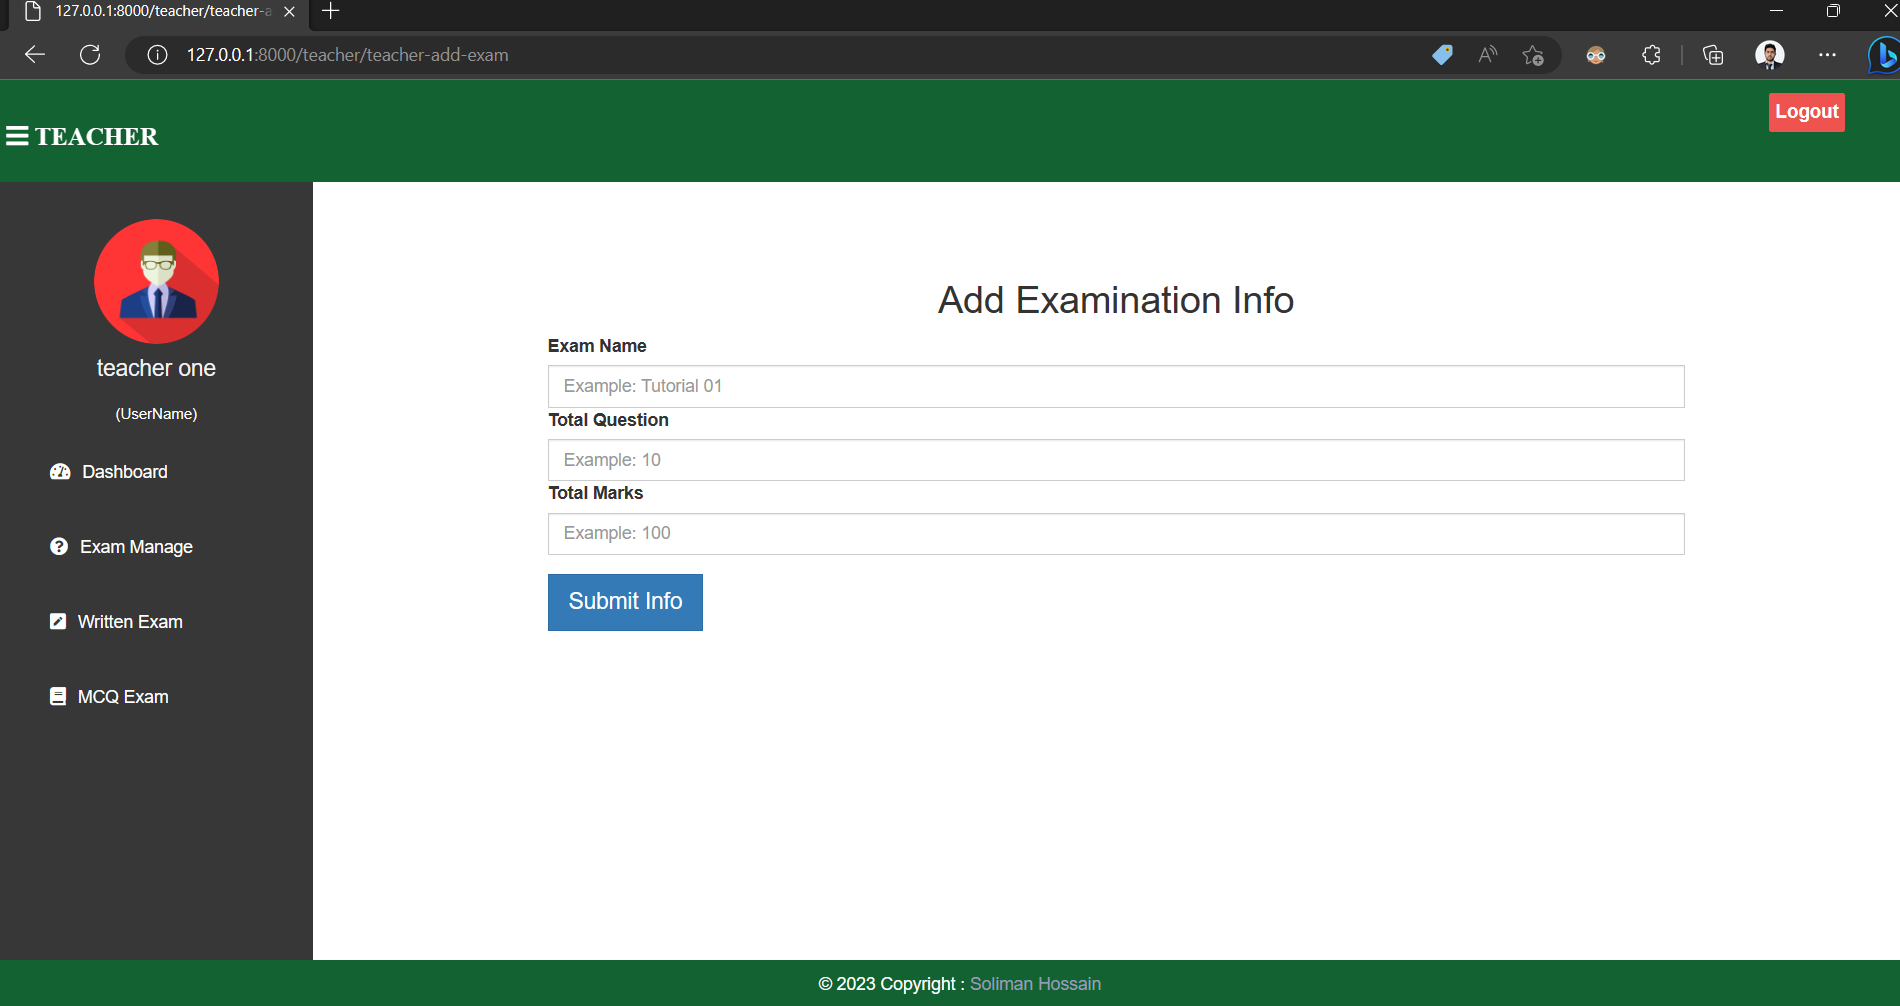
\includegraphics[scale=.35]{img/teacherques.png}
    \caption{Create Exams}
    \label{fig:teacherques}
\end{figure}
The following figure \ref{fig:teacherques} shows it will be possible to add information about the upcoming examination of the student from which they will be able to know which course exam it is, how many questions there will be, total marks of the exams. This information will help them to take better preparation and they will be able to cut a good figure in the exam.
\begin{figure}[H]
    \centering
    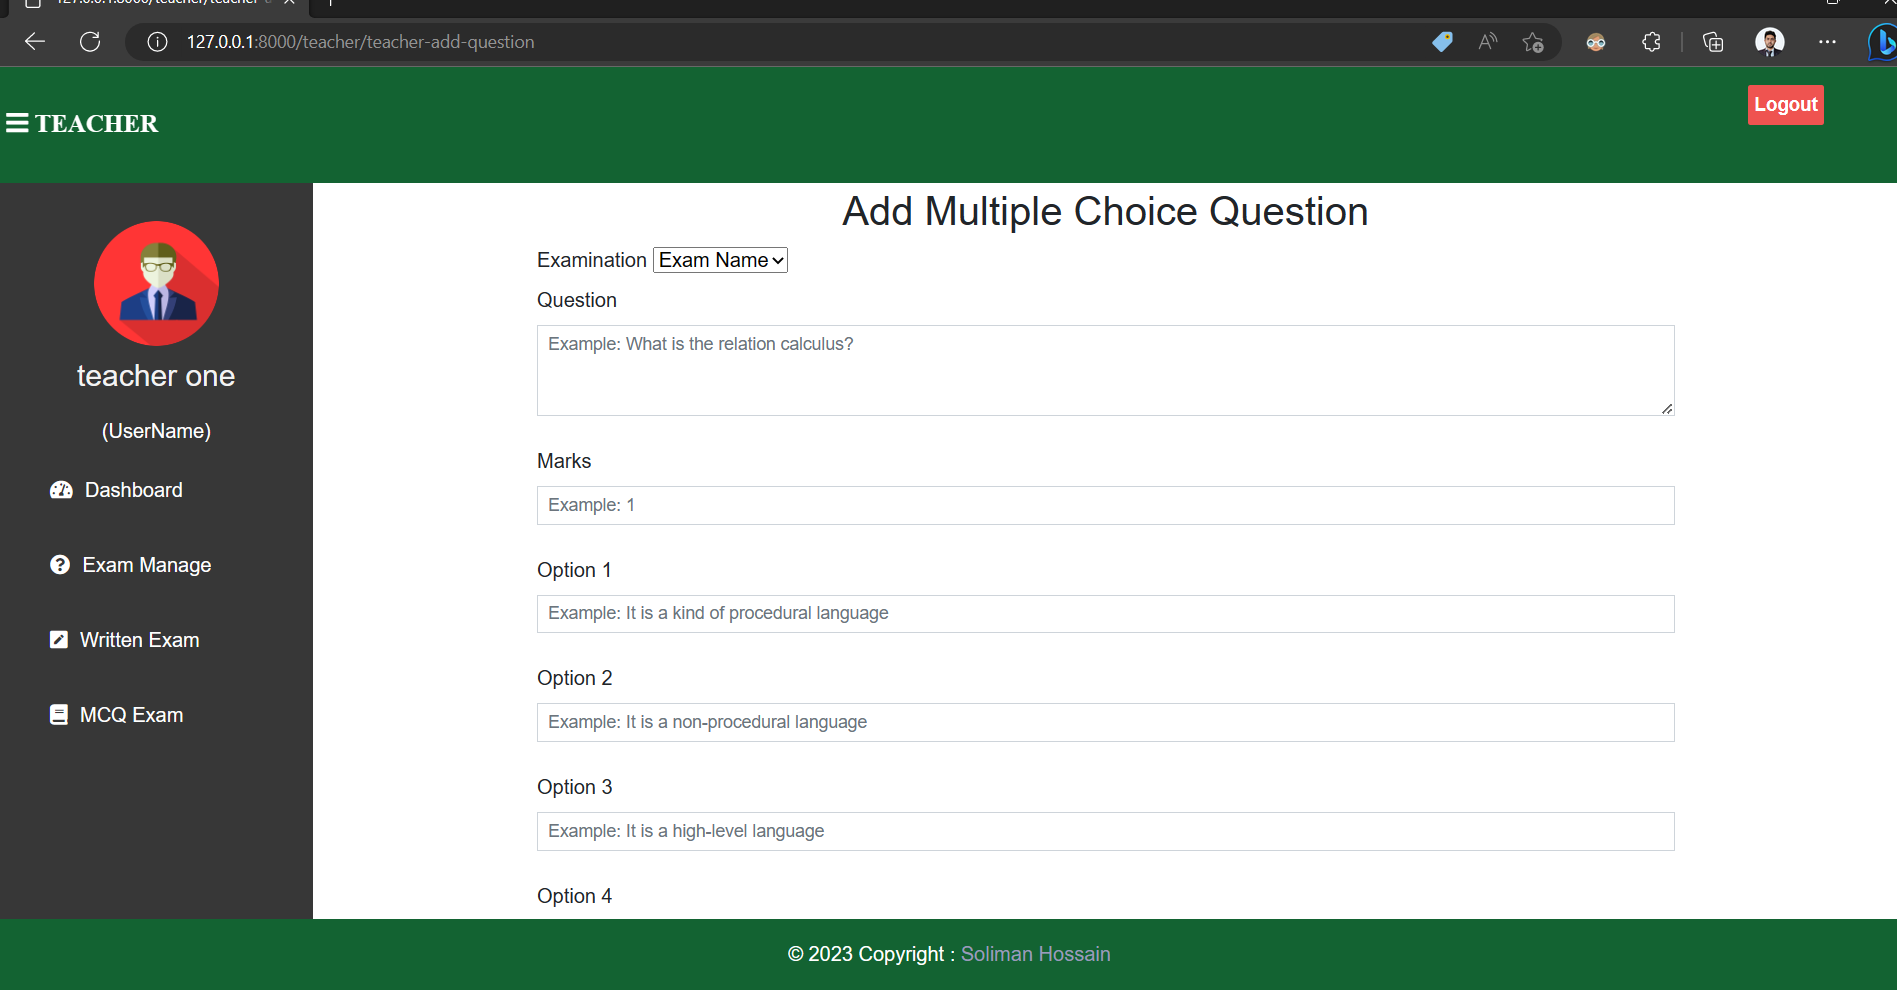
\includegraphics[scale=.36]{img/MCQ.png}
    \caption{Written Exam Question}
    \label{fig:MCQ}
\end{figure}
The teacher will be able to create both written and MCQ questions easily on this platform as it is shown on figure \ref{fig:MCQ}  and \ref{fig:CT} . The written exam questions will be made with lecture content and then upload with question as following:

\begin{figure}[H]
    \centering
    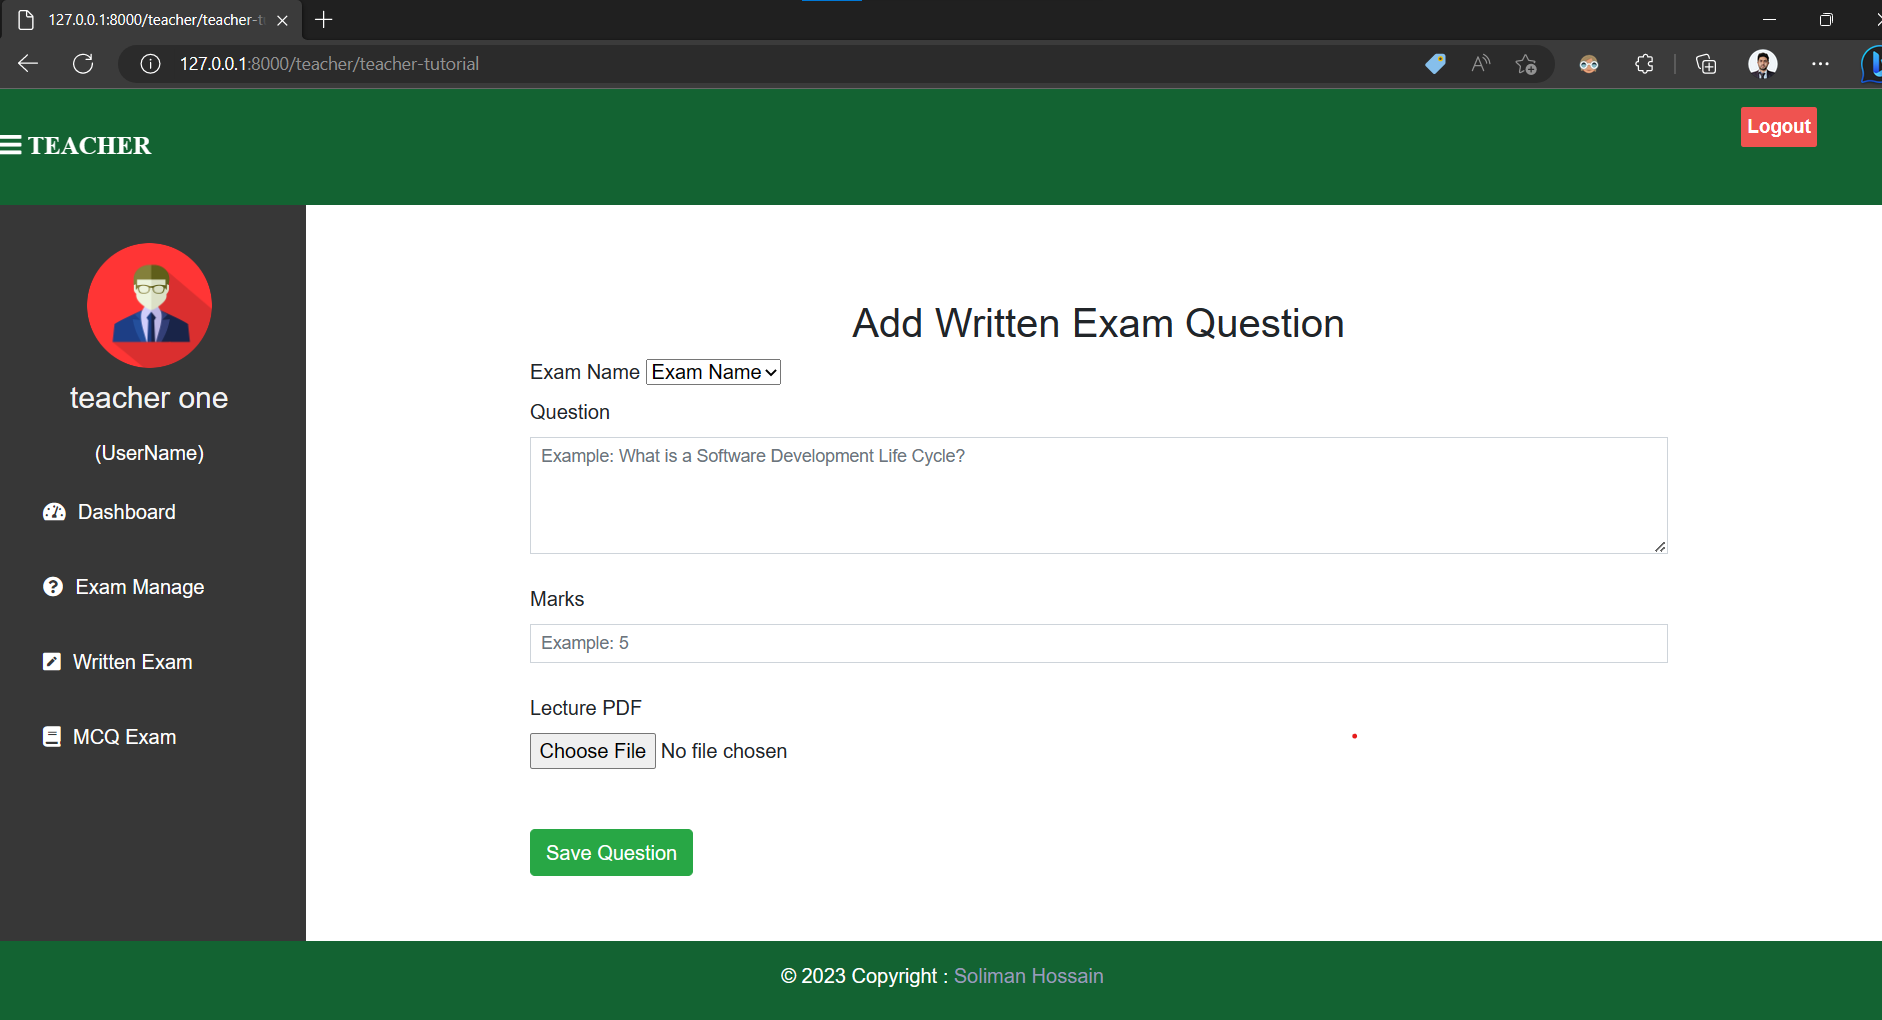
\includegraphics[scale=.36]{img/CT.png}
    \caption{MCQ Exam Question}
    \label{fig:CT}
\end{figure}
The teacher, student and registrar can view the mark-sheet. Teacher and Registrar can see from individual student id and teacher can update it, Registrar can printout and publish result. The mark-sheet of one student as the figure \ref{fig:mark} shows:
\begin{figure}[!h]
    \centering
    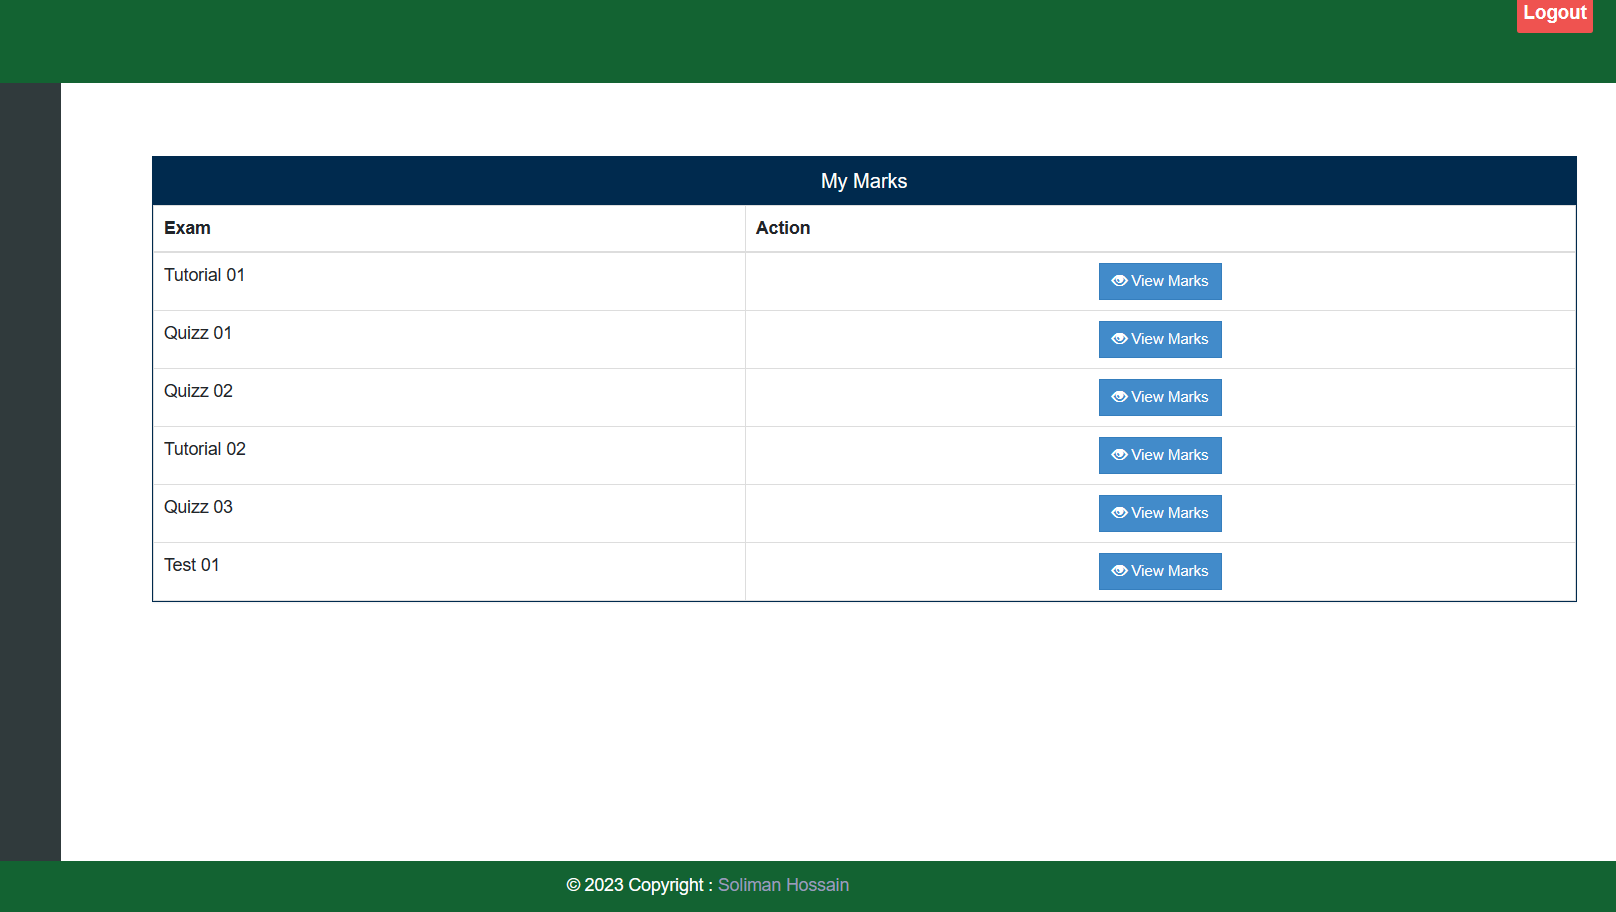
\includegraphics[scale=.4]{img/mark.png}
    \caption{Mark Sheet}
    \label{fig:mark}
\end{figure}

\subsection{Registrar}
The Registrar will have access to follow up both the teachers and the students and also access of their all information. Here the registrar of the institution will act as an admin of the system.
\begin{figure}[H]
    \centering
    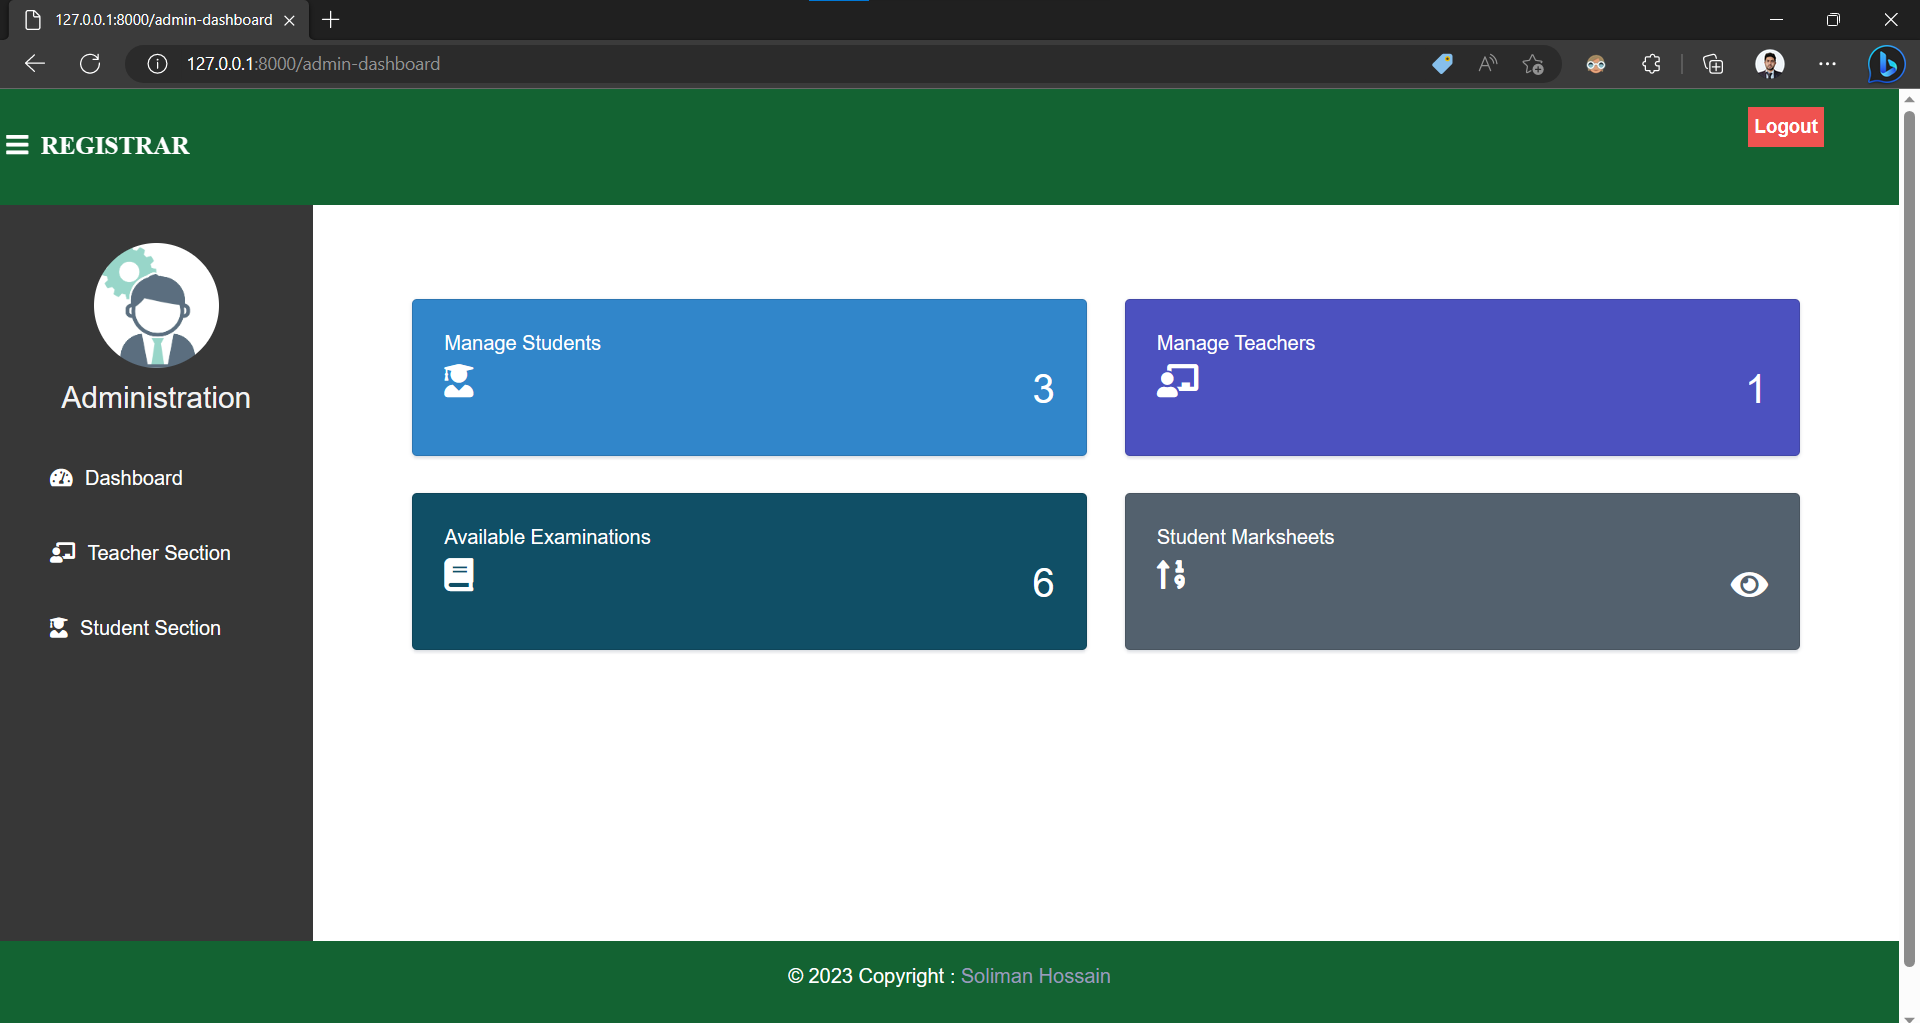
\includegraphics[scale=.36]{img/admin.png}
    \caption{Registrar Dashboard}
    \label{fig:admin}
\end{figure}

 
 In Registrar panel’s dashboard there will be available examinations, manage total number of registered teachers and student and student marksheet as the figure \ref{fig:admin} shows. Where registrar can add or approve, update, remove students and teachers.
Registrar can view all question sets and also marksheet of student which can be printed and published it.
\begin{figure}[H]
    \centering
    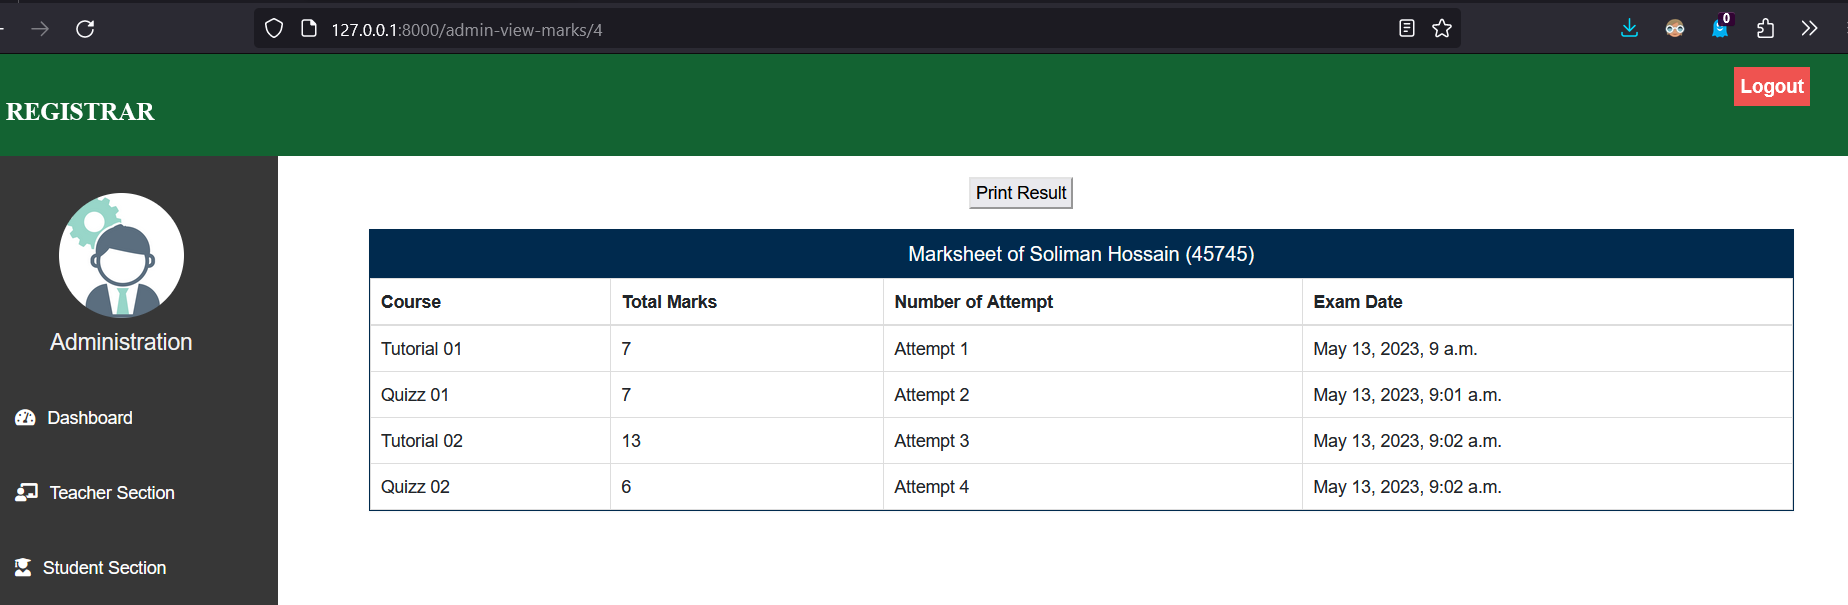
\includegraphics[scale=.36]{img/result.png}
    \caption{Result of a Student}
    \label{fig:result}
\end{figure}



\section{Testing}

This section outlines a comprehensive testing procedure for a web-based student evaluation system. Testing plays a crucial role in ensuring the functionality, reliability, and usability of the system. The procedure covers various aspects of testing to verify that the system meets the requirements and performs as expected.

Experiments were carried out among the students of various batches in order to evaluate the suggested evaluation technique and delivery architecture. A group of 10 students participated in the evaluation processes for the various courses.  The course instructor needed roughly 50 minutes to create an exam that had 8–12 questions, assuming that all the necessary materials were on hand.  After our automated marking system has marked each student's exam paper, the teacher uploads the marking sheet. The students' student accounts can be promptly checked.

These results demonstrate the potency and effectiveness of the distribution architecture and evaluation mechanism that have been suggested. Even employees with modest computer abilities were able to create evaluations more quickly and readily thanks to the system. Additionally, the ability to alter the course structure during the evaluation process gave students the opportunity for individualized and flexible learning.
